\documentclass[11pt,a4paper]{article}

% --- Packages ---
\usepackage[utf8]{inputenc}
\usepackage[T1]{fontenc}
\usepackage{amsmath,amssymb,amsthm}
\usepackage{mathtools}
\usepackage{booktabs}
\usepackage{graphicx}
\usepackage[colorlinks=true,citecolor=blue,linkcolor=blue,urlcolor=blue]{hyperref}
\usepackage{geometry}
\usepackage{setspace}
\usepackage[expansion=false,protrusion=false]{microtype}
\usepackage{tikz}
\usetikzlibrary{shapes,arrows,positioning,fit,calc}
\usepackage{xcolor}

\newtheorem{definition}{Definition}[section]

\geometry{ top=1in, bottom=1in, left=1.1in, right=1.1in }
\setstretch{1.08}

\title{
  \vspace{-1.5cm}
  \textbf{Cerdic Prop Desk: Private, Portfolio-Margined\\[4pt]
  Proprietary Trading on Arc}
  \vspace{-0.3cm}
}

\author{
  Cerdic Protocol Contributors\\[4pt]
  \texttt{https://cerdic.org}
}

\date{}

\begin{document}

\maketitle
\thispagestyle{empty}
\vspace{0.3cm}

\begin{abstract}
  \noindent On-chain proprietary trading firms -- smart contracts that fund a trader
  against pinned, non-retroactive risk rules and pay out on a passed evaluation -- are a
  real, fast-growing category (HyperPNL and comparable platforms), built as a direct
  response to the CeFi prop-firm industry's reputation for changing rules after a trader
  qualifies. Every example live today shares two structural limits: they run on transparent
  order books, so a funded trader's strategy is visible to the firm and to competitors
  in real time, and they margin positions in isolation, wasting the capital efficiency a
  multi-market trader should get from hedged exposure. This paper shows that a prop desk
  is not a new protocol to build -- it is a composition of primitives Cerdic's clearing
  kernel already defines: capability tokens for non-retroactive risk rules, the portfolio
  margin engine for cross-market capital efficiency, TEE-matched execution for strategy
  privacy, and the existing vault performance-fee path for payout. We formalize the model,
  compare it against the current on-chain prop-firm architecture, and give the lifecycle
  and risk analysis for both the firm and the trader.
\end{abstract}

\vspace{0.2cm}
\noindent\textbf{Keywords:} proprietary trading, funded trader programs, portfolio margin,
capability tokens, private execution

\newpage
\tableofcontents
\newpage

%=============================================================================
\section{Introduction}
\label{sec:introduction}
%=============================================================================

A prop firm funds a trader with the firm's capital, not the trader's own, and keeps the
majority of the profit in exchange for taking on the capital risk. The CeFi version of this
industry has a well-known trust problem: a trader passes an evaluation against one set of
rules, and the firm tightens them, disputes a payout, or changes terms after the fact,
because the rules were never anything more than the firm's word.

On-chain prop firms answer this directly. Rules -- daily loss limit, maximum drawdown,
profit target, minimum trading days -- are written into a smart contract at account
creation and cannot be changed while the account is open. HyperPNL and comparable platforms
run this today: a two-phase evaluation (e.g., 10\% profit target / 9\% max drawdown / 5\%
daily loss limit in Phase 1, a lower target with the same risk bounds in Phase 2), with
payout triggered by the contract and settled in seconds once a trader qualifies. This is a
young category -- roughly six months old at the time of writing -- but it is real, live,
and growing.

Every implementation of it today shares two limits that come from the venue it is built on,
not from the prop-firm model itself:

\begin{itemize}
  \item \textbf{Transparency.} These platforms run on public order books. A funded trader's
  size, direction, and open positions are visible to anyone watching the chain -- including
  competitors, and including the firm itself, which can see exactly how a trader is
  positioned before an evaluation resolves.
  \item \textbf{Isolated margin.} Positions are margined per-market. A funded trader running
  a hedged, multi-market book gets no capital-efficiency credit for the hedge -- the same
  gross-margin waste Cerdic's core paper describes for retail traders applies identically
  here, just with the firm's capital instead of the trader's own.
\end{itemize}

\textbf{This paper's claim is narrow and specific:} Cerdic does not need a new subsystem to
support prop trading. The clearing kernel's existing primitives -- capability tokens,
portfolio margin, TEE-matched execution, and vault performance-fee settlement -- already
compose into a prop desk that keeps the non-retroactive-rules property the category is
built around, while removing both structural limits above.

%=============================================================================
\section{Background: The On-Chain Prop-Firm Pattern}
\label{sec:background}
%=============================================================================

\subsection{Why rules are pinned, not just published}

The defining feature of the category is not that risk rules exist -- CeFi prop firms
publish rules too -- it is that the rules are enforced by code the firm cannot unilaterally
change once a trader's account is open. This is the entire trust proposition: a trader who
passes evaluation under a specific drawdown limit knows that limit was fixed before they
started, and no update, dispute process, or after-the-fact reinterpretation can move it.

\subsection{Typical parameters}

\begin{table}[h]
  \centering
  \begin{tabular}{ll}
    \toprule
    \textbf{Parameter} & \textbf{Typical range (2026 on-chain prop firms)} \\
    \midrule
    Profit target & 5\%--10\% (often lower in a second phase) \\
    Daily loss limit & 4\%--5\% \\
    Max drawdown & 8\%--10\%, trailing \\
    Minimum trading days & Firm-specific, sometimes waived \\
    Payout settlement & On-chain, seconds, in USDC \\
    \bottomrule
  \end{tabular}
  \caption{Representative risk parameters from current on-chain prop-firm platforms.}
  \label{tab:params}
\end{table}

\subsection{What the venue determines, not the model}

Both limits identified in Section~\ref{sec:introduction} are properties of the underlying
exchange, not of the prop-firm contract layered on top of it. A prop-firm contract sitting
on a transparent, isolated-margin perp DEX inherits that DEX's transparency and margin
inefficiency regardless of how well-designed its own risk-rule logic is. This is the gap
Cerdic's kernel closes -- not by building a better prop-firm contract, but by being a
venue where the prop-firm layer inherits privacy and portfolio margin for free.

%=============================================================================
\section{The Prop Desk Model}
\label{sec:model}
%=============================================================================

A prop desk on Cerdic is a specific configuration of four primitives already defined in
the core clearing kernel -- nothing here is a new contract type.

\begin{table}[h]
  \centering
  \begin{tabular}{lp{9.2cm}}
    \toprule
    \textbf{Prop-firm requirement} & \textbf{Existing Cerdic primitive} \\
    \midrule
    Risk rules pinned at account creation, non-retroactive &
      Capability token -- signed once by the firm's owner key over the scoped action fields,
      kernel-verified, cannot be re-signed to tighten terms on an open account \\
    Daily loss limit / max drawdown / position caps &
      Agent execution policy -- max position size, max leverage, daily loss limit, cooldown
      periods, all kernel-enforced, not left to the trader's own code \\
    Capital efficiency across a hedged book &
      Portfolio margin engine -- $f_K$ prices a genuine hedge as a margin credit
      (core paper, portfolio margin section), giving a funded trader real efficiency an
      isolated-margin venue cannot \\
    Strategy privacy from the firm and competitors &
      TEE-matched execution -- the firm sets and enforces the risk rules without ever
      seeing the trader's live positions; only settlement events are visible on-chain \\
    Payout on passing evaluation / profit split &
      Vault performance-fee settlement path -- structurally the same mechanism as a
      strategy vault manager's fee, reused rather than rebuilt \\
    \bottomrule
  \end{tabular}
  \caption{The prop desk is a composition, not a new subsystem.}
  \label{tab:composition}
\end{table}

\begin{definition}[Prop account]
A prop account is a clearing account $A_{\text{prop}} = (\mathcal{B}, \mathcal{P},
\mathcal{H})$ funded entirely by the firm's capital allocation, associated with a capability
$$\text{capability} = \text{Sign}_{sk_{\text{firm}}}\big(H(\text{trader\_id}, \text{limits},
\text{expiry})\big)$$
where $\text{limits}$ encodes the evaluation's risk parameters (Table~\ref{tab:params}) as
kernel-enforced execution-policy fields, not as advisory terms. The signature is produced
once, at account creation; the kernel accepts trader actions only while a valid, unexpired
capability with these exact limits exists, and the firm has no on-chain action that
modifies $\text{limits}$ for an open account.
\end{definition}

%=============================================================================
\section{Lifecycle}
\label{sec:lifecycle}
%=============================================================================

\begin{figure}[h]
  \centering
  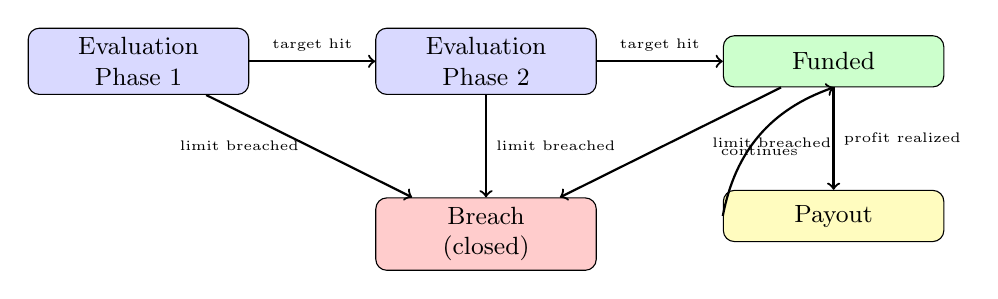
\begin{tikzpicture}[
    state/.style={rectangle, rounded corners, draw, minimum width=2.8cm, minimum height=0.65cm, align=center, font=\small},
    arrow/.style={->, thick}
  ]
    \node[state, fill=blue!15] (eval1) {Evaluation\\Phase 1};
    \node[state, fill=blue!15, right=1.6cm of eval1] (eval2) {Evaluation\\Phase 2};
    \node[state, fill=green!20, right=1.6cm of eval2] (funded) {Funded};
    \node[state, fill=yellow!25, below=1.3cm of funded] (payout) {Payout};
    \node[state, fill=red!20, below=1.3cm of eval2] (breach) {Breach\\(closed)};

    \draw[arrow] (eval1) -- node[above, font=\tiny] {target hit} (eval2);
    \draw[arrow] (eval2) -- node[above, font=\tiny] {target hit} (funded);
    \draw[arrow] (funded) -- node[right, font=\tiny] {profit realized} (payout);
    \draw[arrow, bend left] (payout.west) to node[below, font=\tiny] {continues} (funded.south);
    \draw[arrow] (eval1) -- node[left, font=\tiny] {limit breached} (breach);
    \draw[arrow] (eval2) -- node[right, font=\tiny] {limit breached} (breach);
    \draw[arrow] (funded) -- node[right, font=\tiny, xshift=0.4cm] {limit breached} (breach);
  \end{tikzpicture}
  \caption{Prop account state machine. Every transition is a kernel-enforced check against
  the capability's pinned limits (Section~\ref{sec:model}) -- the firm observes state
  transitions, not the positions that caused them.}
  \label{fig:lifecycle}
\end{figure}

\textbf{Evaluation phases.} The trader operates the prop account under the pinned execution
policy. Portfolio margin is computed exactly as for any other account (core paper, portfolio
margin section) -- a hedged evaluation trader gets the same $f_K$ credit a funded trader
would, which matters because evaluation performance under isolated margin materially
understates what the same strategy could do once funded on a portfolio-margined venue.

\textbf{Breach.} A daily-loss or drawdown breach is a kernel-level check against
$\mathcal{C}_{\text{eff}}$ and realized/unrealized PnL, evaluated the same way a liquidation
threshold is (core paper, liquidation mechanism). The account closes; capital returns to the
firm's pool. No dispute process exists because no discretion exists -- the check is a
comparison against the pinned limits, not a judgment call.

\textbf{Funded and payout.} Passing both phases moves the account into funded status with
the firm's full allocation. Payout uses the existing vault performance-fee settlement path:
realized profit above the firm's retained share settles to the trader on the same schedule
a vault would distribute returns, denominated in USDC, at Arc's native settlement speed.

%=============================================================================
\section{Privacy: What the Firm Sees}
\label{sec:privacy}
%=============================================================================

The central departure from the existing category is what the firm's own contract is able to
observe. On a transparent venue, the firm (and everyone else) can watch a trader's live
book while an evaluation is in progress -- which means the firm can, in principle, see
exactly how close a trader is to a limit before the trader does, and a competing firm can
copy a strategy mid-evaluation. On Cerdic, the firm's capability token grants and enforces
limits without granting visibility: the TEE matches the trader's orders privately (core
paper, private matching section), and the only things that reach the chain -- and therefore
the firm -- are state transitions (Figure~\ref{fig:lifecycle}) and the collateral/PnL
numbers needed to check a breach, not the position set that produced them. A trader is
risk-limited by rules they cannot see removed, and private from a firm that cannot see their
strategy. Neither property trades off against the other, because they are enforced by two
different mechanisms -- the capability token for limits, the TEE for confidentiality -- that
do not depend on each other.

%=============================================================================
\section{Capital Efficiency}
\label{sec:efficiency}
%=============================================================================

Consider a funded trader running a EURC/USDC hedge alongside a BTC/USDC directional
position (once a second, correlated market exists on Cerdic per the core paper's roadmap).
Under isolated margin -- the model every current on-chain prop firm uses -- the trader posts
full margin on both legs independently. Under Cerdic's portfolio margin,
$f_K(\mathcal{P}) = \beta \sum \rho_{ij} s_i s_j$ prices the genuine offset as a margin
credit. The firm's capital backs the same trader activity with less locked collateral,
which is a direct improvement in how much trading a fixed capital allocation can support --
not a new feature, simply the core paper's leverage moat applied to a funded account instead
of a self-funded one.

%=============================================================================
\section{Risk Analysis}
\label{sec:risk}
%=============================================================================

\textbf{Firm risk.} The firm's maximum loss on a given prop account is bounded by the
pinned execution policy, enforced at the kernel level rather than trusted to the trader's
own discipline or code -- the same enforcement model already described for agent accounts
generally (core paper, agent security section). A compromised or malicious trader cannot
exceed the daily loss limit or max drawdown any more than a compromised agent can exceed its
capability's scope elsewhere in the system.

\textbf{Trader risk.} The trader's protection is that the limits cannot be tightened after
the capability is signed -- the core trust property the entire category exists to provide,
here inherited directly from the capability-token design rather than re-implemented.

\textbf{Shared risk.} Both parties inherit the core paper's stated risks generally: oracle
dependency for breach/liquidation checks, TEE hardware trust for the privacy property, and
smart contract risk in the kernel itself (core paper, Section~1.4 and security analysis).
Nothing about the prop desk composition introduces a new risk category -- it inherits
exactly the kernel's existing risk surface, which is the point of building it as a
composition rather than new infrastructure.

%=============================================================================
\section{Relation to the Core Protocol}
\label{sec:relation}
%=============================================================================

This is an application-layer pattern, not a protocol change. It requires no new kernel
contracts beyond what the core paper already specifies for agent accounts, portfolio
margin, TEE matching, and strategy vaults. It depends on: agent accounts with capability
tokens (core paper, agent-native section, MVP), the full portfolio margin engine (MVP),
working TEE-matched execution (MVP), and institutional sub-account isolation for the firm's
capital pool (core paper roadmap, Phase 3). A minimal single-trader version -- one firm
account, one capability, no sub-account hierarchy -- is reachable as soon as the MVP's
agent-account and portfolio-margin pieces exist; the multi-trader, multi-desk version
follows institutional sub-accounts in Phase 3.

%=============================================================================
\section{Conclusion}
\label{sec:conclusion}
%=============================================================================

On-chain prop trading is a real category solving a real trust problem -- non-retroactive,
code-enforced risk rules -- but every current implementation inherits its venue's
transparency and isolated-margin limits. Cerdic does not need to build a competing
prop-firm product; its clearing kernel already contains every primitive the category
depends on, plus two properties -- strategy privacy and portfolio margin -- that no current
on-chain prop firm has. A prop desk is simply what those primitives look like composed for
this specific use case.

\end{document}
